%!TEX root=seke.tex
% mainfile: ../seke.tex

To gain a more nuanced understanding of the results, we construct a
regression tree using the \textit{ctree} package for the R langauge. A
regression tree attempts to use the values of predictor variables to
predict the value of a responce variable. A regression tree accopmlishes
this by repeadidily splitting the data according to what predictor varaible has the
most influcence on the response varaible. Each node in the tree represents a choice
of predictor varaible, and the level of the node indicates its
importance to the prediction---higher being more important.

\textit{ctree} produced the tree shown as Figure~\ref{fig:atree} to
predict the runtime of \textit{SchemaAnalyst} with the predictor varaibles:
tables, columns, UNIQUEs, NOT NULLs, CHECKs, Criterion, and
DataGenerator. The regression tree confirms that the number of
tables has the largest impact on runtime, and also reveals that when the number of tables in the schema is small, 
the choice of coverage criterion is the most important predictor for runtime.

Another invocation of \textit{ctree}, excluding tables from the list of
predictors, confirmed that when the number of tables in the schema is small, the choice of coverage criterion is the
most important predictor for runtime, followed by the choice of data
generator, and then the number of columns in the schema.

While the trees provide insight into the relative impact of each
predictor on the runtime of \textit{SchemaAnalyst}, the box and whisker
plots produced as the leaves of the trees do not provide a detailed view
of the choices within each predictor.  To gain a finer level of
granularity, we produce box and wisker plots of our own.

\begin{figure*}
\centering
  \centering
  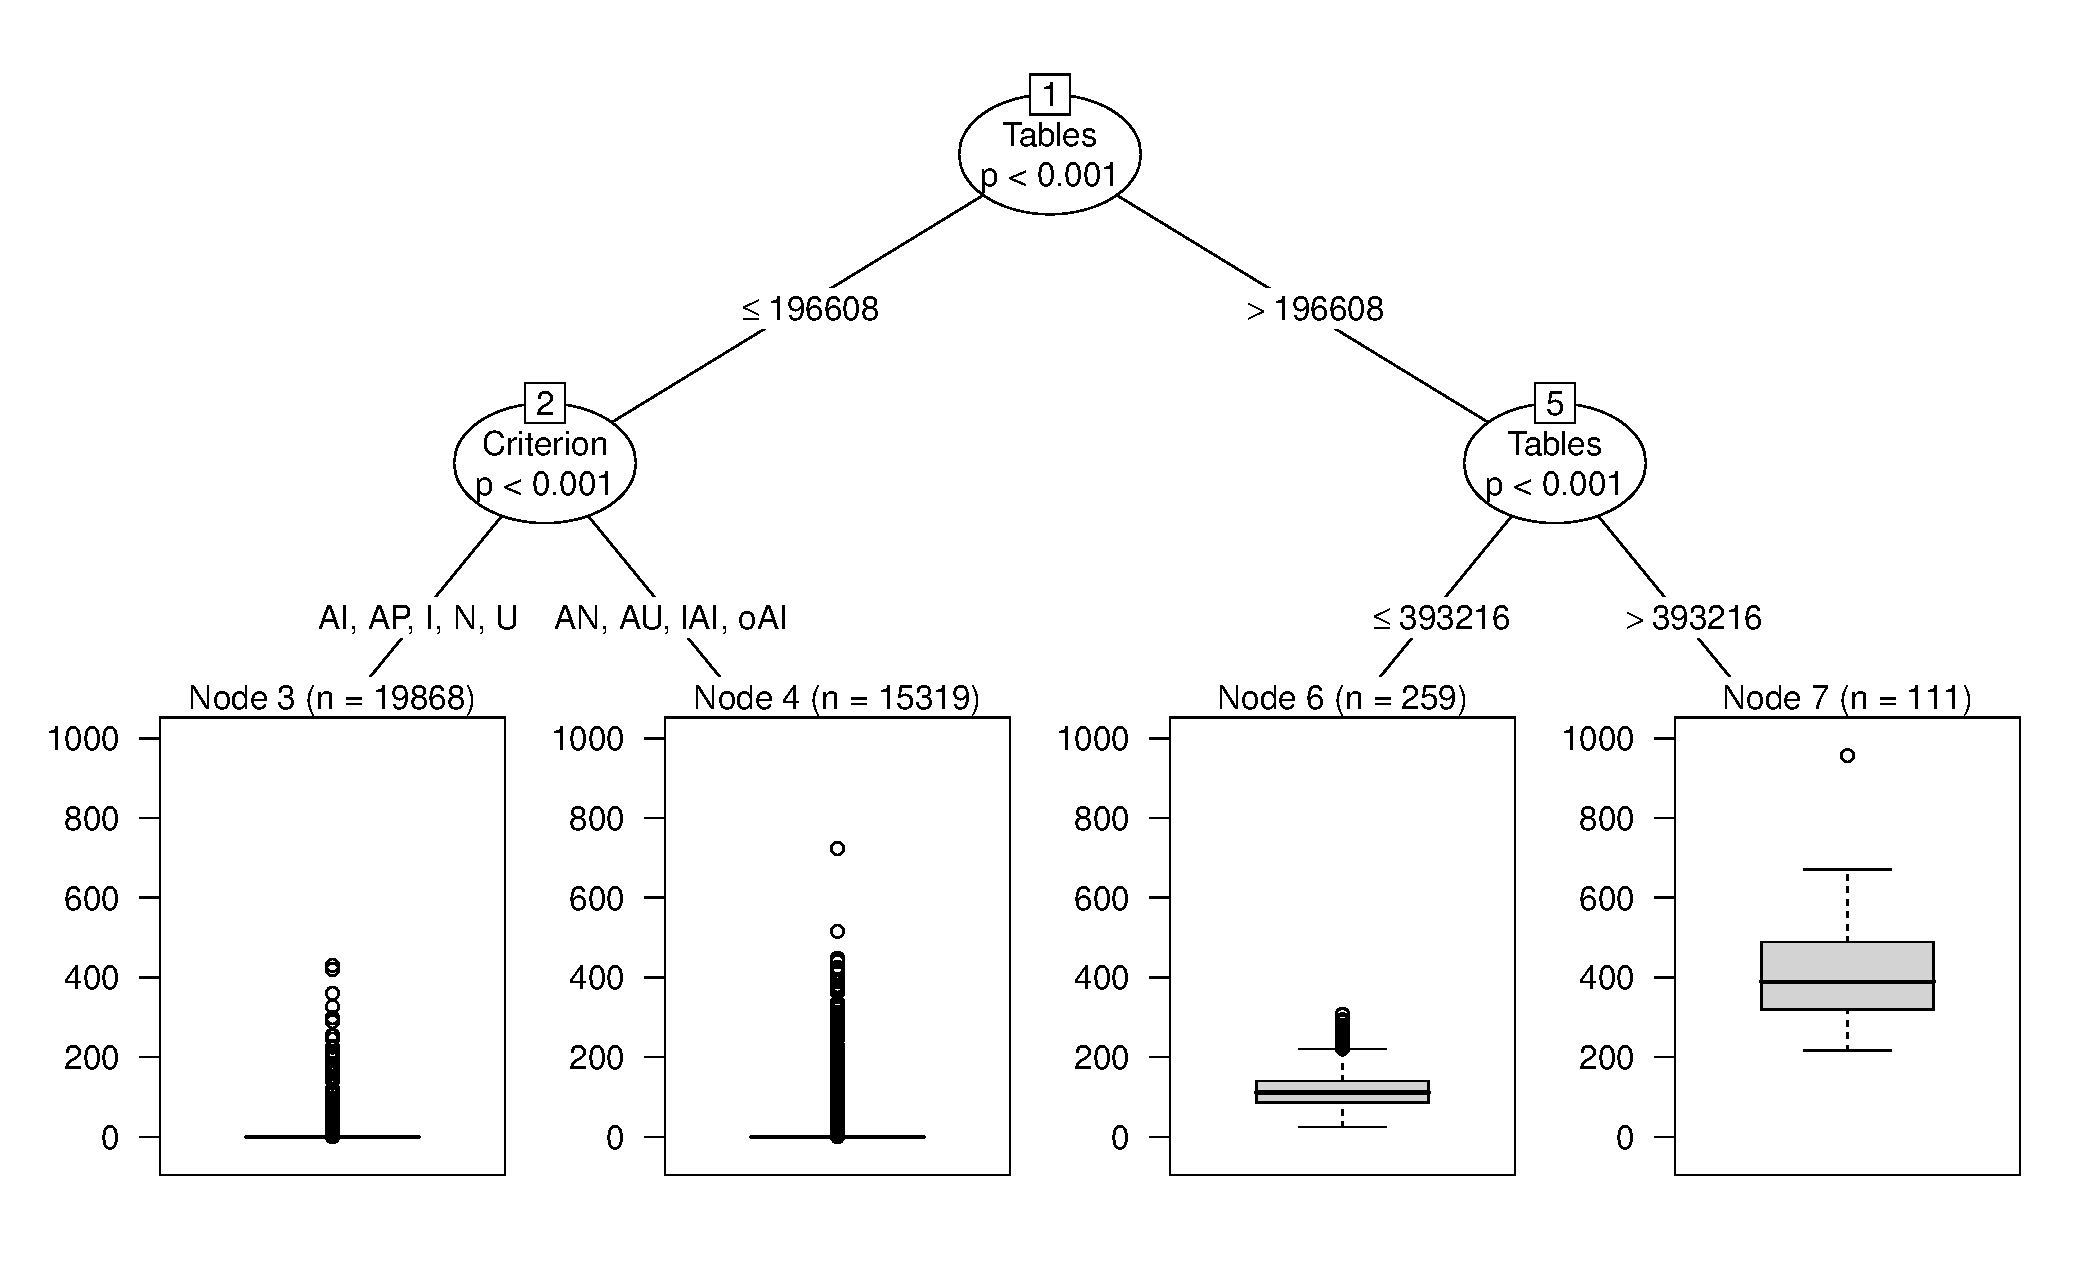
\includegraphics[width=.75\linewidth]{diagrams/AllTree.pdf}
  \caption{Regression tree using all variables to predict runtime in
  minutes. \vspace{-.15in}}
  \label{fig:atree}
  \vspace{-.15in}
\end{figure*}

\begin{figure*}
\centering
  \centering
  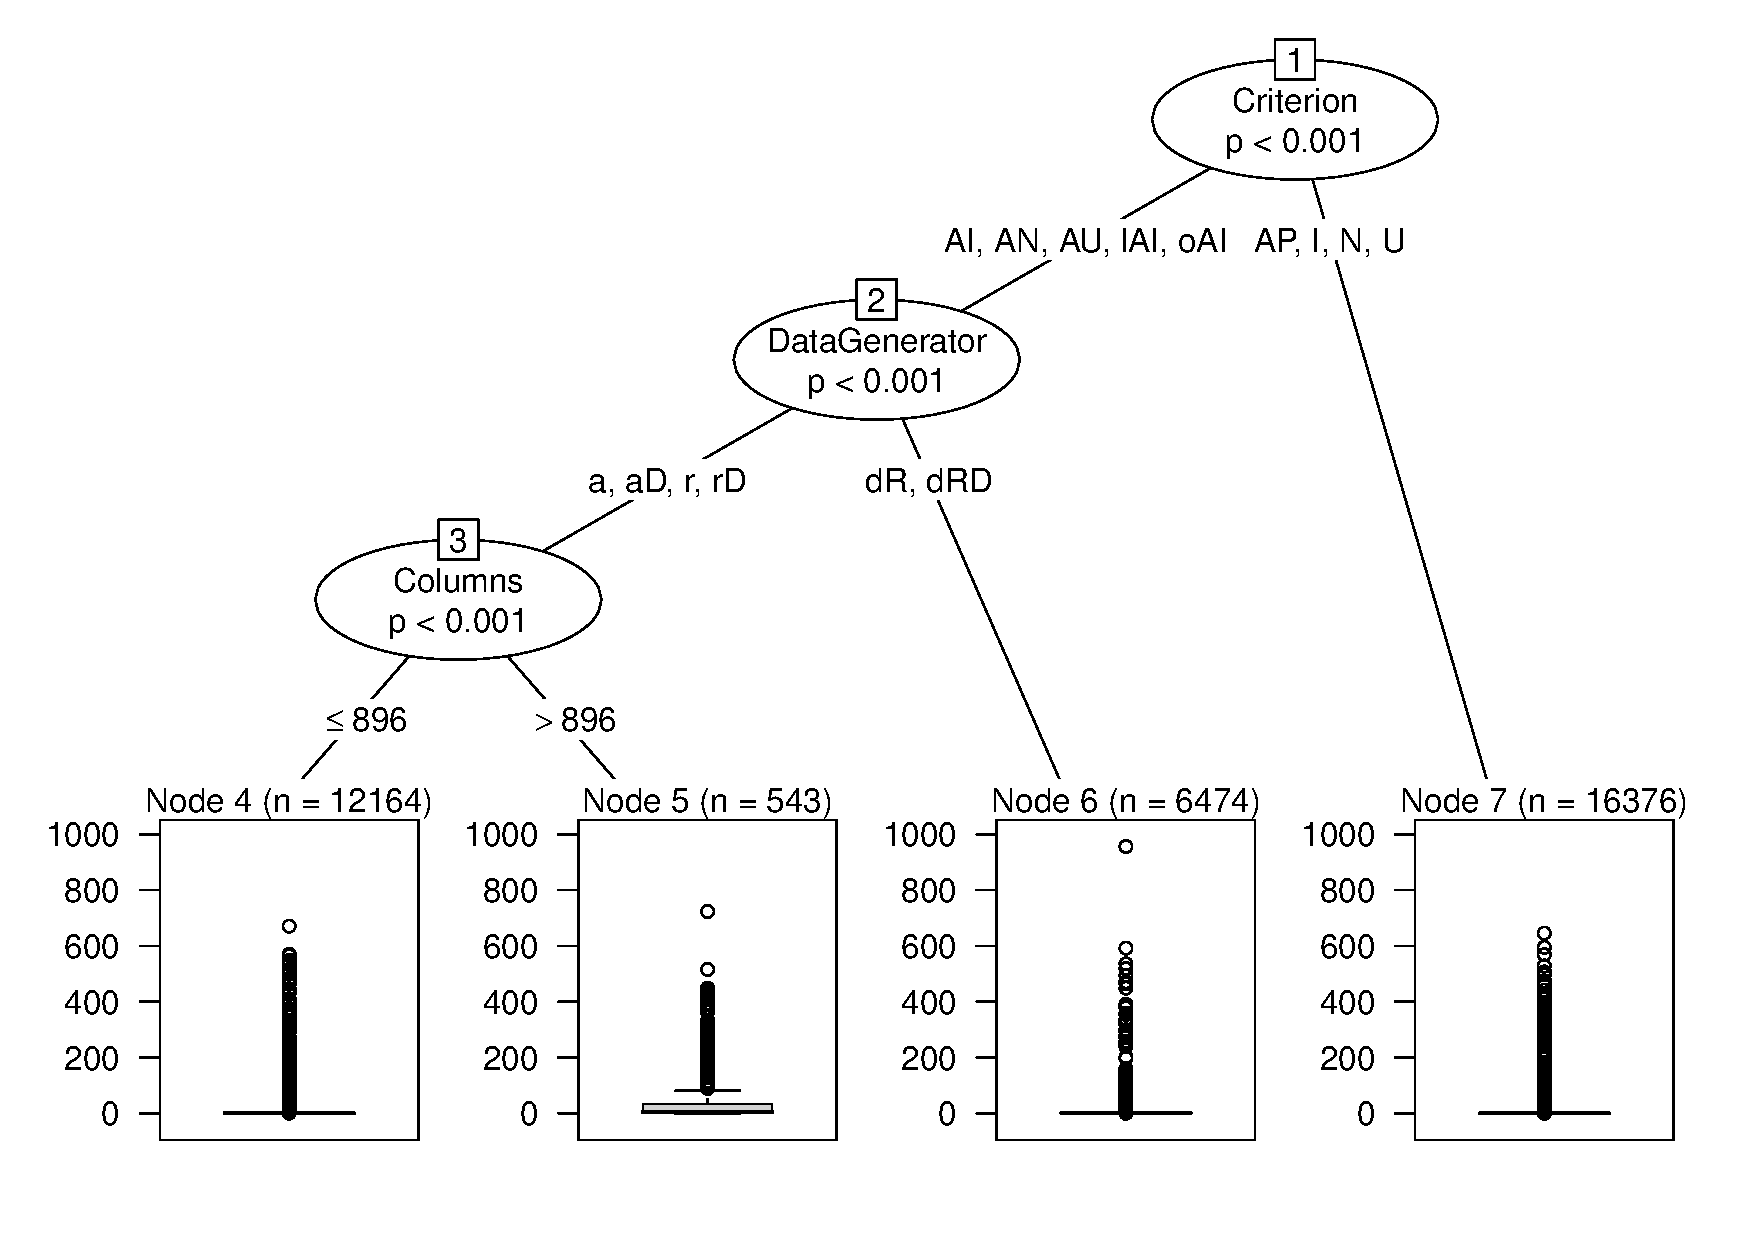
\includegraphics[width=.75\linewidth]{diagrams/NoTableCtreesd.pdf}
  \caption{Regression tree predicting runtime excluding Tables.\vspace{-.15in}}
  \label{fig:ttree}
  \vspace{-.15in}
\end{figure*}
